\documentclass[11pt,a4paper]{article}
\usepackage[margin=2.3cm]{geometry}
\usepackage{amsmath,amssymb,bm}
\usepackage{graphicx}
\usepackage{booktabs,array}
\usepackage[table]{xcolor}
\usepackage{microtype}
\usepackage{caption}
\usepackage{enumitem}
\usepackage[most]{tcolorbox}
\usepackage[numbers,sort&compress]{natbib}
\usepackage[colorlinks=true,linkcolor=blue!50!black,citecolor=green!40!black,urlcolor=blue!60!black]{hyperref}
\numberwithin{equation}{section}
\graphicspath{{../figures/}}
\captionsetup{font=small,labelfont=bf}
\setlist{itemsep=2pt,topsep=3pt}
\newcommand{\sq}{\sqrt{f_R}}
\newcommand{\dd}{\mathrm{d}}
\newcommand{\jh}{\hat\jmath_\ell}
\newcommand{\RR}{\mathcal R}
\newcommand{\TT}{\mathcal T}
\definecolor{qcol}{RGB}{235,104,52}
\definecolor{icol}{RGB}{42,120,214}
\definecolor{lcol}{RGB}{27,175,122}
\newtcolorbox{question}{colback=qcol!6,colframe=qcol!80!black,boxrule=0.6pt,arc=2pt,left=6pt,right=6pt,top=3pt,bottom=3pt,
  fonttitle=\bfseries\small,title=Question}
\newtcolorbox{keyidea}{colback=icol!6,colframe=icol!80!black,boxrule=0.6pt,arc=2pt,left=6pt,right=6pt,top=3pt,bottom=3pt,
  fonttitle=\bfseries\small,title=Key idea}
\newtcolorbox{learned}{colback=lcol!6,colframe=lcol!70!black,boxrule=0.6pt,arc=2pt,left=6pt,right=6pt,top=3pt,bottom=3pt,
  fonttitle=\bfseries\small,title=What we learned}
\sloppy

\title{\textbf{Gravitational waves and a spherical thin shell}\\[4pt]
\large A step-by-step account: why the shell must have pressure, how it enters the wave equation,\\
how much it reflects, how it rings, and why it is unstable}
\author{Final project, gravitational-wave course}
\date{September 2026}

\begin{document}
\maketitle

\begin{abstract}
We study gravitational perturbations of the simplest horizonless compact object: a thin spherical shell of matter
at areal radius $R>2M$, with flat space inside and Schwarzschild spacetime of mass $M$ outside. We compute the
reflection and transmission coefficients $\RR(\omega)$, $\TT(\omega)$ and the quasinormal modes (QNMs) for odd (axial)
and even (polar) parity. The paper is written as a chain of questions, each motivated by the answer to the previous
one. (1) Can the shell be static? A domain wall or a dust shell cannot; a perfect-fluid shell can, with a pressure
fixed by its compactness. (2) How does the shell enter the wave equation? For odd parity it is a repulsive
$\delta$-function of strength $\Delta=\sq(1-\sq)/R$. For even parity it is a frequency-dependent $2\times2$ transfer
matrix that conserves flux exactly. (3) How much does it reflect? It reflects everything at low frequency and nothing
at high frequency ($\RR\simeq\Delta^2/4\omega^2$), and it approaches the black-hole reflectivity as $R\to2M$. (4) How
does it ring? Through cavity modes, long-lived trapped modes for $R<3M$ (the origin of echoes), and oscillations of the
shell matter. None of these tends to the black-hole QNMs. (5) Is the static shell stable? No. One even-parity matter
mode grows exponentially, in agreement with Pitre, Schneider and Poisson (2026) and with a Newtonian calculation. The
growth is slow compared with the waves, so the scattering results for the fluid shell remain meaningful. A domain wall
frozen at its turning point is not a controlled approximation for even parity. All results are checked by two
numerical methods, by known limits and by a time-domain simulation.
\end{abstract}

\tableofcontents
\newpage

%==========================================================================================
\section*{Reading guide: the line of thought in eight steps}
\addcontentsline{toc}{section}{Reading guide: the line of thought in eight steps}
The whole project is one argument. Each step answers a question and raises the next.
\begin{enumerate}[label=\textbf{Step \arabic*.},leftmargin=4.2em]
\item \textbf{Background} (Sec.~\ref{sec:bg}). Scattering at fixed frequency needs a static background. \emph{Can a shell
be static?} Only with a positive surface pressure $p=\kappa(R)\sigma$. This selects the \emph{fluid shell} (model C). The
domain wall of the prior notes must be \emph{frozen} at its turning point (model A).
\item \textbf{Waves on each side} (Sec.~\ref{sec:pert}). Away from the shell the equations are standard: Regge--Wheeler
and Zerilli outside, the flat wave equation inside. One subtlety: the interior clock is slow, so $\nu=\omega/\sq$.
\item \textbf{Junction conditions} (Sec.~\ref{sec:junction}). All the physics of the shell is in how the two solutions
are glued. Odd parity gives a $\delta$-barrier. Even parity gives a $2\times2$ matrix, because the shell moves and its
matter oscillates.
\item \textbf{Scattering} (Sec.~\ref{sec:scatt}). The closed system reflects everything. To measure how much the
\emph{object} reflects we open the interior, as a horizon would. Then $\RR+\TT=1$, and the limits
$\omega\to0$, $\omega\to\infty$ and $R\to2M$ can be understood analytically.
\item \textbf{Numerics and trust} (Sec.~\ref{sec:num}). Two independent methods, known limits, energy balance and
black-hole benchmarks.
\item \textbf{Ringing} (Sec.~\ref{sec:qnm}). The QNMs fall into cavity modes, trapped modes and matter modes. A
time-domain simulation shows them directly.
\item \textbf{Stability} (Sec.~\ref{sec:matter}). One matter mode is purely imaginary and growing: the static shell is
unstable. Its Newtonian origin is derived analytically.
\item \textbf{Back to Step 1} (Sec.~\ref{sec:backto1}). Is the background slow enough for Steps 3--6 to make sense? For
the fluid shell, yes. For the frozen wall, no, and its even-parity results are ambiguous.
\end{enumerate}
Units: $G=c=1$. Frequencies are in units of $M^{-1}$ and the time dependence is $e^{-i\omega t}$. $[X]=X_+-X_-$ is the
jump across the shell (outside minus inside), and $f_R=1-2M/R$.

%==========================================================================================
\section{Introduction}\label{sec:intro}
A black hole responds to a gravitational perturbation in a well-understood way. The odd and even perturbations obey
the Regge--Wheeler \cite{RW57} and Zerilli \cite{Zerilli70} equations. Low-frequency waves are reflected by the
potential barrier and high-frequency waves are absorbed by the horizon \cite{Vishveshwara70}. The final ringing is a
discrete set of QNMs \cite{Leaver85,KokkotasSchmidt99,Nollert99,BCS09,KonoplyaZhidenko11}. Horizonless compact objects
(``black-hole mimickers'' such as gravastars \cite{MazurMottola04,VisserWiltshire04,ChirentiRezzolla07,Pani09}) behave
differently for two reasons. They have a \emph{surface}, where the perturbation must satisfy junction conditions, and an
\emph{interior}, where waves can be trapped. Their ringdown can therefore contain ``echoes''
\cite{Cardoso2016PRL,Cardoso2016PRD,Abedi2017,CardosoPani2019}.

The simplest such object is a thin shell of matter. Birkhoff's theorem and regularity at the centre force the interior
to be flat \cite{ondas}, and the exterior is Schwarzschild. The shell is a timelike hypersurface $\Sigma$ carrying a
surface stress tensor $S_{ab}$. The Lanczos--Israel formalism \cite{Lanczos24,Israel66,Poisson04,IS84} relates $S_{ab}$
to the jump of extrinsic curvature across $\Sigma$. Two prior notes \cite{ondas,burbuja} had solved the interior wave
equation and set up this formalism for a \emph{domain wall}. In doing so they ran into an obstacle: such a wall cannot
be static. This paper resolves the obstacle and carries the calculation through.

\paragraph{Relation to the literature.} During the work we found that the static fluid shell (our model C) was studied
recently by Pitre, Schneider and Poisson \cite{PSP26} (PSP26). They computed its QNMs with a different formalism and
found it dynamically unstable, complementing an eikonal analysis by Yang, Bonga and Pan \cite{YBP23}. We reproduce
their results and use them as a validation. As far as we know, the following are new: the reflection and transmission
coefficients, the explicit $\delta$-function form of the odd junction, and the analysis of the frozen domain wall.

%==========================================================================================
\section{Step 1 --- The background: can a thin shell stand still?}\label{sec:bg}
\begin{question}
A scattering calculation at fixed frequency $\omega$ assumes that the object does not change in time. The prior notes
found that a domain wall always collapses. Which shells, if any, admit a static configuration?
\end{question}

\subsection{Thin-shell formalism}
Let $\Sigma$ have intrinsic coordinates $y^a=(\tau,\theta,\phi)$ and unit normal $n_\alpha$ pointing from the interior
($-$) to the exterior ($+$). The induced metric and the extrinsic curvature are \cite{Poisson04}
\begin{equation}
h_{ab}=g_{\alpha\beta}e^\alpha_ae^\beta_b,\qquad K_{ab}=e^\alpha_ae^\beta_b\nabla_\alpha n_\beta ,
\end{equation}
with $e^\alpha_a=\partial x^\alpha/\partial y^a$. The two junction conditions are \cite{Israel66}, \cite{Poisson04}
(Eqs.~3.49, 3.56), \cite{IS84} (Eq.~2.6):
\begin{equation}
[h_{ab}]=0,\qquad [K_{ab}]-h_{ab}[K]=-8\pi S_{ab}.
\label{eq:israel}
\end{equation}
In words, the geometry of the shell is the same seen from both sides, and the \emph{bending} of the shell differs
between the two sides by an amount set by its matter. For a perfect fluid,
$S^{ab}=\sigma u^au^b+p(h^{ab}+u^au^b)$, with surface energy density $\sigma$ and surface pressure $p$. Ipser and
Sikivie use the tension $\tau=-p$. A domain wall has $\tau=\sigma$, i.e.\ $S_{ab}=-\sigma h_{ab}$ \cite{IS84}.

\subsection{Spherical shell and its equation of motion}
Inside, $\dd s^2=-\dd T^2+\dd r^2+r^2\dd\Omega^2$. Outside, $\dd s^2=-f\dd t^2+f^{-1}\dd r^2+r^2\dd\Omega^2$ with $f=1-2M/r$.
For a shell $r=R(\tau)$ define $\alpha=\sqrt{1+\dot R^2}$ and $\beta=\sqrt{f(R)+\dot R^2}$. The extrinsic curvatures are
(IS84 3.5--3.6; Poisson 3.65)
\begin{equation}
K^\theta{}_\theta\big|_+=\frac{\beta}{R},\quad K^\theta{}_\theta\big|_-=\frac{\alpha}{R},\qquad
K^\tau{}_\tau\big|_+=\frac{\ddot R+M/R^2}{\beta},\quad K^\tau{}_\tau\big|_-=\frac{\ddot R}{\alpha}.
\end{equation}
Inserting them into Eq.~\eqref{eq:israel} gives
\begin{align}
\sigma&=\frac{\alpha-\beta}{4\pi R}\qquad\Longleftrightarrow\qquad M=\tfrac12(\alpha+\beta)\,4\pi\sigma R^2,\label{eq:mass}\\
(\alpha+\beta)\ddot R&=-\frac{\alpha M}{R^2}+\frac{2p}{\sigma}\,\frac{\alpha\beta(\alpha+\beta)}{R}.\label{eq:eom}
\end{align}
These are IS84's Eqs.~(3.7a) and (3.8). The mass formula~\eqref{eq:mass} says that $M$ is the rest mass of the shell
corrected by its kinetic and gravitational binding energy. The equation of motion~\eqref{eq:eom} reads like
Newton's law: gravity (first term) always pulls inward, and pressure pushes outward only if $p>0$.

\subsection{The four options}
\begin{keyidea}
Set $\dot R=\ddot R=0$ in Eq.~\eqref{eq:eom}. Gravity must be balanced by pressure, and there is exactly one ratio
$p/\sigma$ that does it. Everything else collapses.
\end{keyidea}
With $\alpha=1$ and $\beta=\sq$,
\begin{equation}
\frac{p}{\sigma}=\kappa(R)=\frac{1-\sq}{4\sq},\qquad \sigma=\frac{1-\sq}{4\pi R},\qquad p=\frac{(1-\sq)^2}{16\pi R\sq}
\label{eq:kappa}
\end{equation}
(Poisson 3.80--3.81). The options for the model are then:
\begin{itemize}
\item \textbf{Domain wall} ($p=-\sigma$). Both terms of~\eqref{eq:eom} are negative, so the wall always collapses to a
black hole: ``a spherical wall with $\tau\ge0$ always collapses to a black hole, regardless of its size'' \cite{IS84}. The
best one can do is to \emph{freeze} it at its turning point $\dot R=0$, where
\begin{equation}
\ddot R=-\frac{1+3\sq}{2R}.
\label{eq:Rdd}
\end{equation}
We call this \textbf{model A}. It is an approximation, valid only if the waves oscillate much faster than the wall
moves.
\item \textbf{Dust} ($p=0$). Then $(\alpha+\beta)\ddot R=-\alpha M/R^2<0$, and a static dust shell does not exist. (The
relation $M=4\pi\sigma R^2\sq$ suggested in the task statement is incompatible with the angular junction condition
$4\pi\sigma R=1-\sq$ unless $M=0$.)
\item \textbf{Static perfect fluid} with $p=\kappa(R)\sigma$: \textbf{model C}, our primary model. It is an exact
static solution. The ratio $\kappa$ is not a free parameter: it is fixed by $R/M$, so the family has one parameter, the
compactness (Table~\ref{tab:bg}). The dominant energy condition $p\le\sigma$ gives $\kappa\le1$, i.e.\
$R\ge25M/12\simeq2.08M$.
\item \textbf{de Sitter interior} (gravastar \cite{Pani09}). Not treated. Model C is its flat-interior, $\sigma\ne0$
relative.
\end{itemize}

\paragraph{Equation of state for perturbations.} A static background fixes $p$ but not how $p$ responds when the shell
is compressed. Following PSP26 \cite{PSP26} we take a barotropic shell with adiabatic index $\Gamma$:
\begin{equation}
\delta p=\Gamma\,\frac{p}{\sigma+p}\,\delta\sigma\equiv v_s^2\,\delta\sigma,\qquad v_s^2=\frac{\Gamma\kappa}{1+\kappa},
\label{eq:eos}
\end{equation}
with fiducial value $\Gamma=2$. Causality, $v_s^2\le1$, gives the same bound $R\ge25M/12$ for $\Gamma=2$. Only even
perturbations compress the shell, so only they depend on $\Gamma$.

\begin{table}[h]\centering\small
\caption{Background quantities of models C and A. $\omega_{\rm dyn}=\sq(|\ddot R|/R)^{1/2}$ is the wall's collapse rate in
exterior time; $(M/R^3)^{1/2}$ sets the scale of the fluid shell's matter modes.}\label{tab:bg}
\resizebox{\textwidth}{!}{\begin{tabular}{rrrrrrrrr}\toprule
$R/M$ & $\sigma M$ & $pM$ & $\kappa=p/\sigma$ & $v_s^2(\Gamma{=}2)$ & I\&S (3.7a) resid. & $\ddot R_{\rm wall}M$ & $\omega_{\rm dyn}M$ & $(M/R^3)^{1/2}M$\\\midrule
2.2 & 0.02527 & 1.463e-02 & 0.5792 & 0.7335 & 0.00e+00 & -0.4328 & 0.1337 & 0.3065 \\
3.0 & 0.01121 & 2.052e-03 & 0.1830 & 0.3094 & 1.39e-17 & -0.4553 & 0.2249 & 0.1925 \\
6.0 & 0.00243 & 1.367e-04 & 0.0562 & 0.1064 & 0.00e+00 & -0.2875 & 0.1787 & 0.0680 \\
10.0 & 0.00084 & 2.479e-05 & 0.0295 & 0.0573 & 1.73e-18 & -0.1842 & 0.1214 & 0.0316 \\
\bottomrule\end{tabular}
}
\end{table}

\begin{learned}
A static thin shell with flat interior \emph{must} have positive surface pressure, $p/\sigma=(1-\sq)/4\sq$. We use this
fluid shell (model C) as the primary model. We also keep the domain wall frozen at its turning point (model A), and we
check in Step 8 whether that freezing is justified.
\end{learned}

%==========================================================================================
\section{Step 2 --- Waves on each side of the shell}\label{sec:pert}
\begin{question}
What equations do gravitational perturbations obey inside and outside the shell, and how are the two sides related?
\end{question}

\subsection{The interior clock runs slow}
On a static shell the two metrics must induce the same geometry, so $\dd T=\sq\,\dd t$. A perturbation
$\propto e^{-i\omega t}$ outside is therefore $\propto e^{-i\nu T}$ inside, with
\begin{equation}
\nu=\omega/\sq .
\label{eq:nu}
\end{equation}
Waves are \emph{blueshifted} inside. (The prior notes and the task statement wrote $\jh(\omega r)$. The correct
argument is $\nu r$, as also in PSP26.) A convenient \emph{global tortoise coordinate} is
\begin{equation}
x=r+2M\ln(r/2M-1)\quad (r>R),\qquad x=x_R+(r-R)/\sq\quad (r<R),
\label{eq:x}
\end{equation}
in which both regions obey $-\partial_t^2\Psi+\partial_x^2\Psi-V(x)\Psi=0$.

\subsection{Master functions}
Following Martel and Poisson \cite{MP05} (MP05), we use gauge-invariant master functions: the
Cunningham--Price--Moncrief function $\Psi_{\rm odd}$ \cite{CPM78} and the Zerilli--Moncrief function $\Psi_{\rm even}$
\cite{Moncrief74}. Outside the shell both obey
\begin{equation}
\frac{\dd^2\Psi}{\dd r_*^2}+\big[\omega^2-V(r)\big]\Psi=0,\qquad
V_{\rm RW}=f\Big[\frac{\ell(\ell+1)}{r^2}-\frac{6M}{r^3}\Big],\qquad
V_{\rm Z}=f\,\frac{2n^2(n+1)r^3+6n^2Mr^2+18nM^2r+18M^3}{r^3(nr+3M)^2},
\label{eq:master}
\end{equation}
with $n=(\ell-1)(\ell+2)/2$ (RW57 Eq.~25; Zerilli Eq.~5; MP05 4.26, 5.15). Inside, $M=0$ and both potentials reduce to
$\ell(\ell+1)/r^2$ \cite{ondas}:
\begin{equation}
\Psi''+\Big[\nu^2-\frac{\ell(\ell+1)}{r^2}\Big]\Psi=0\quad\Longrightarrow\quad
\Psi_{\rm int}=A\,\jh(\nu r),\qquad \jh(z)=zj_\ell(z)\simeq\frac{z^{\ell+1}}{(2\ell+1)!!},
\label{eq:int}
\end{equation}
the regular Riccati--Bessel function \cite{AS72,DLMF}. Both parities have the same interior profile and differ only in
the junction conditions. For the scattering problem we also need the Riccati--Hankel functions
$\hat h^{\rm out/in}_\ell=-\hat y_\ell\pm i\jh\sim e^{\pm i(z-\ell\pi/2)}$.

\paragraph{Reconstructing the metric.} The junction conditions are written in terms of metric components, so we need
them in terms of $\Psi$. In vacuum the odd sector gives (Regge--Wheeler gauge $h_2=0$)
\begin{equation}
h_t=\frac f2\,\partial_r(r\Psi_{\rm odd}),\qquad h_r=-\frac{i\omega r}{2f}\Psi_{\rm odd},
\label{eq:oddrecon}
\end{equation}
and the even sector, in the gauge $j_a=G=0$ with $H_0=H_2\equiv H$ and $\mu=(\ell-1)(\ell+2)$, gives
\begin{equation}
K=f\,\Psi'+\frac{\mu(\mu+2)r^2+6\mu Mr+24M^2}{2r^2(\mu r+6M)}\,\Psi,\qquad
H_1=-i\omega\Big[r\,\Psi'+\frac{\mu r^2-3\mu Mr-6M^2}{(r-2M)(\mu r+6M)}\,\Psi\Big],
\end{equation}
and
\begin{equation}
H=f\,\frac{\mu r^2-3\mu Mr-6M^2}{(r-2M)(\mu r+6M)}\,\Psi'+\Big[\frac{Q(r)}{2r^2(r-2M)(\mu r+6M)^2}-\frac{\omega^2r}{f}\Big]\Psi,
\end{equation}
with $Q=\mu^2(\mu+2)r^4-2M\mu^2(\mu-1)r^3-12M^2\mu(\mu-3)r^2-72M^3(\mu-1)r-144M^4$. These relations were obtained by
linearizing the Einstein tensor symbolically. All field equations are satisfied identically, and $V_{\rm Z}$
reproduces MP05's (4.26).

\paragraph{The potential landscape.} Figure~\ref{fig:pot} shows the resulting 1D problem: the flat centrifugal barrier
inside, the RW/Zerilli barrier outside, and the shell between them. The Chandrasekhar transformation \cite{Chandrasekhar83}
maps RW solutions into Zerilli solutions outside. This is why a black hole has the same spectrum for both parities.
With a shell present, the two parities have different junction conditions and the spectra split.

\begin{figure}[t]\centering
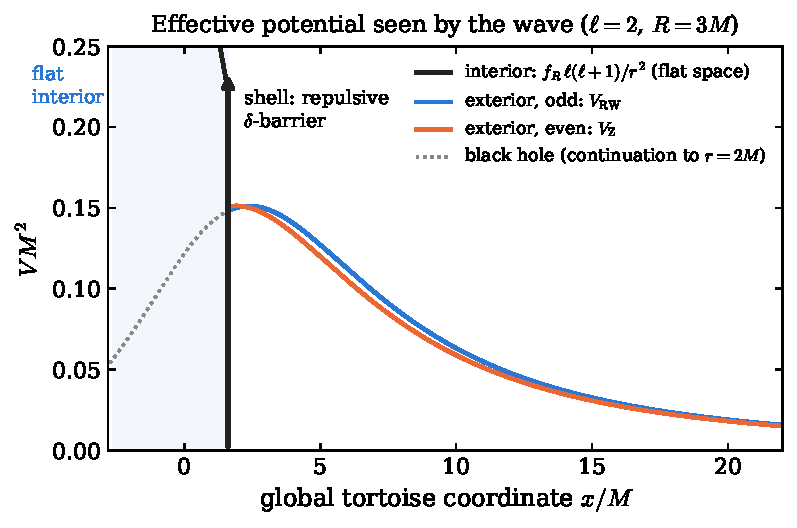
\includegraphics[width=0.72\textwidth]{r3_f01_potential.pdf}
\caption{The problem in one picture: potential seen by an $\ell=2$ wave for a shell at $R=3M$, in the global tortoise
coordinate~\eqref{eq:x}. The arrow marks the shell, which for odd parity is a $\delta$-barrier (Sec.~\ref{sec:odd}).
Dotted: what a black hole would have instead of the shell and the flat interior.}\label{fig:pot}
\end{figure}

\begin{learned}
Away from the shell the problem is standard. The only new ingredients are the blueshift $\nu=\omega/\sq$ and the
way $\Psi$ is continued across $r=R$. That continuation is the subject of Step 3.
\end{learned}

%==========================================================================================
\section{Step 3 --- The shell in the wave equation: linearized junction conditions}\label{sec:junction}
\begin{question}
How are $\Psi_-(R)$ and $\Psi_-'(R)$ inside related to $\Psi_+(R)$ and $\Psi_+'(R)$ outside? The prior notes had computed
one component of the perturbed extrinsic curvature and left open how the background term $[K]^{(0)}$ enters.
\end{question}

\subsection{Strategy}
\begin{keyidea}
Perturb Eq.~\eqref{eq:israel} to first order. The perturbation on each side is written in that side's own
Regge--Wheeler gauge, which is convenient for the master functions but not adapted to the shell. The shell therefore
appears to sit at \emph{different} perturbed positions when seen from the two sides. We allow for this explicitly
through a perturbed embedding on each side.
\end{keyidea}
Concretely, $x^\mu_\pm(y)=X^\mu_{0\pm}(y)+\epsilon Z^\mu_\pm(y)$, with $Z_+=(0,\xi_+Y,0,0)$ and
$Z_-=(\zeta Y,\xi_-Y,\eta\,\partial_\theta Y,0)$, plus an angular shift in the odd sector (cf.\ Pani et al.\ \cite{Pani09},
App.~A). Here $\xi_\pm$ are the radial displacements of the shell in the two gauges, and $\zeta,\eta$ describe how the
time and angles are identified. The shell matter is perturbed too: $\sigma\to\sigma+\delta\sigma\,Y$,
$p\to p+v_s^2\delta\sigma\,Y$, plus a tangential velocity $U$. The procedure is:
\begin{enumerate}
\item compute the normal, $h_{ab}$ and $K_{ab}$ to first order on each side, including the displacement of background
fields, $Q(X_0+\epsilon Z)\simeq Q(X_0)+\epsilon Z^\mu\partial_\mu Q$;
\item project onto spherical harmonics and replace the metric functions by $\Psi$ with Eqs.~\eqref{eq:oddrecon} ff.;
\item impose Eq.~\eqref{eq:israel}. This gives a linear system $\mathsf A(\omega)\bm x=\mathsf B(\omega)(\Psi_-,\Psi_-')^{\rm T}$
for the unknowns $\bm x=(\text{shell variables},\Psi_+,\Psi_+')$;
\item solve it. The last two components define the transfer matrix $\mathsf T$:
$(\Psi_+,\Psi_+')^{\rm T}=\mathsf T(\Psi_-,\Psi_-')^{\rm T}$.
\end{enumerate}
All of this was done with symbolic algebra (SymPy) and cross-checked by hand in the odd sector.

\subsection{Odd parity: the shell is a $\delta$-function barrier}\label{sec:odd}
Odd perturbations do not change $g^{rr}$ and do not move the shell radially, so the normal keeps its background form.
The perturbed extrinsic curvature is
\begin{equation}
\delta K_{tA}=\frac{\sqrt f}{2}\big(\partial_rh_t-\partial_th_r\big)X_A,\qquad \delta K_{AB}=-\sqrt f\,h_r\,X_{AB},
\end{equation}
where the first expression is Eq.~(12) of the prior notes \cite{burbuja}. Three conditions remain:
\begin{enumerate}
\item \emph{$AB$ component.} $\delta S_{AB}=0$ for odd parity, so $[\sq\,h_r]=0$. With Eq.~\eqref{eq:oddrecon} and
$\nu=\omega/\sq$ this is exactly $\Psi_+=\Psi_-$. \emph{The blueshift is what makes $\Psi$ continuous.}
\item \emph{$\tau A$ component.} This is where the prior notes stopped. It contains $[K]^{(0)}$ and the matter velocity
$U$. The background term combines with the pressure term as $[K]^{(0)}-8\pi p=-4\pi\sigma$. All dependence on $p$, and
hence on $\ddot R$ for the wall, cancels identically, and the equation reduces to $U=0$. \emph{Odd waves do not move
the shell's matter.}
\item \emph{Continuity of $\delta h_{\tau A}$.} This gives $(r\Psi_-)'|_R=\sq\,(r\Psi_+)'|_R$.
\end{enumerate}
Combining the three,
\begin{equation}
\boxed{\ \Psi_+=\Psi_-,\qquad \sq\,\Psi_+'-\Psi_-'=\frac{1-\sq}{R}\,\Psi=4\pi\sigma\,\Psi\ }
\quad\Longleftrightarrow\quad\Big[\frac{\dd\Psi}{\dd x}\Big]=\Delta\,\Psi,\qquad \Delta=\frac{\sq(1-\sq)}{R}=4\pi\sigma\sq .
\label{eq:odd}
\end{equation}
\begin{keyidea}
For axial waves the shell is simply a \emph{repulsive $\delta$-potential} $\Delta\,\delta(x-x_R)$ in the 1D wave equation.
Its strength is the surface density times the redshift factor. It is independent of $\omega$, of the equation of state
and of the model (wall or fluid).
\end{keyidea}
The transfer matrix is $\mathsf T_{\rm odd}=\begin{pmatrix}1&0\\(1-\sq)/(R\sq)&1/\sq\end{pmatrix}$, with
$\det\mathsf T_{\rm odd}=f_R^{-1/2}$. Four checks support Eq.~\eqref{eq:odd}:
\begin{itemize}
\item \emph{Literature.} It agrees with PSP26 Eq.~(5.23) and with the matching conditions $[h_0]=0$, $[\sqrt h\,h_1]=0$ of
Pani et al.\ (3.29, A35).
\item \emph{Transparent limit.} As $M\to0$ it reduces to continuity of $\Psi$ and $\Psi'$, the ``inviscid'' limit of
Boyanov et al.\ \cite{Boyanov25}.
\item \emph{Thick-shell derivation.} For axial perturbations of a smooth, static, anisotropic fluid the master potential
is $e^{2\Phi}[\ell(\ell+1)/r^2-6m/r^3+4\pi(\rho-p_r)]$ (App.~\ref{app:axial}; cf.\ \cite{ChandrasekharFerrari91,ThorneCampolattaro67,Kojima92}).
For a layer with $p_r=0$ whose thickness goes to zero, the term $4\pi\rho e^{2\Phi}$ becomes exactly
$\Delta\,\delta(x-x_R)$.
\item \emph{Numerical thick shell.} The mismatch between a numerical thick shell and the thin-shell junction goes to
zero linearly in the thickness, and does so for no alternative value of $\Delta$ (Fig.~\ref{fig:thick}).
\end{itemize}

\begin{figure}[t]\centering
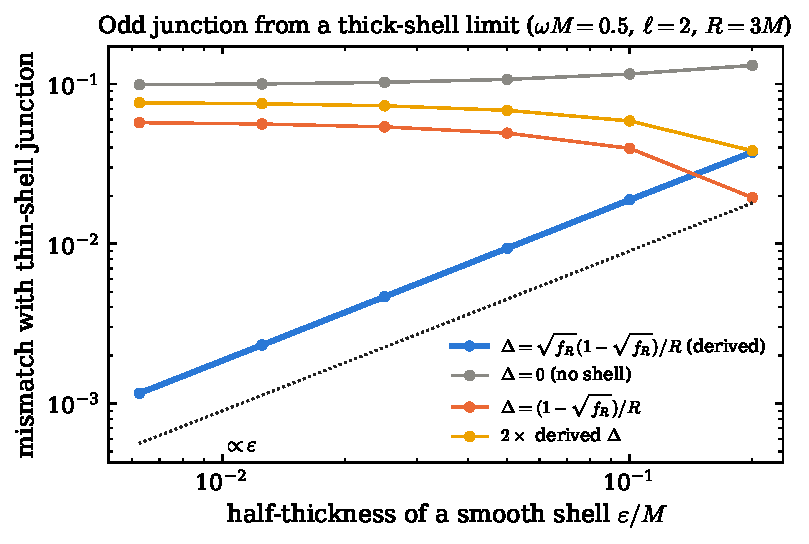
\includegraphics[width=0.66\textwidth]{r3_f09_thick_shell.pdf}
\caption{Odd junction from a thick-shell limit. A smooth shell of half-thickness $\varepsilon$ is compared with thin-shell
junctions of different strength. Only the derived $\Delta$ is approached, linearly in $\varepsilon$.}\label{fig:thick}
\end{figure}

\subsection{Even parity: a $2\times2$ transfer matrix}\label{sec:even}
Even perturbations do move the shell. Continuity of the induced metric forces $\zeta=\eta=0$ and leaves
\begin{equation}
H_+-\frac{2M}{R(R-2M)}\xi_+=H_-,\qquad RK_++2\xi_+=RK_-+2\xi_-,
\end{equation}
in agreement with Pani et al.\ (A16, A20). Since $\xi_+\ne\xi_-$, the shell is displaced by different amounts in the two
gauges. This is why the even junction cannot reduce to a single scalar jump condition. The four Israel components
($\tau\tau$, $\tau A$, trace and trace-free $AB$) involve the matter perturbations
$\delta S_{\tau\tau}=\delta\sigma-\sigma\,\delta h_{\tau\tau}$, $\delta S_{\tau A}=-(\sigma+p)U+p\,\delta h_{\tau A}$,
$\delta S^{\rm tr}_{AB}=v_s^2\delta\sigma R^2+p\,\delta h^{\rm tr}_{AB}$ and $\delta S^{\rm tf}_{AB}=p\,\delta h^{\rm tf}_{AB}$.
For model C this gives 8 equations for 8 unknowns $(\xi_+,\xi_-,\zeta,\eta,\delta\sigma,U,\Psi_+,\Psi_+')$, of full rank.
The solution defines $\mathsf T^{\rm C}_{\rm even}(\omega;\ell,R/M,\Gamma)$. Its properties are:
\begin{itemize}
\item $\Psi$ is \emph{discontinuous} across the shell, and $\mathsf T$ is a full matrix that depends on $\omega$ (through
the shell's inertia) and on the equation of state (through $v_s^2$);
\item $\det\mathsf T=f_R^{-1/2}$ \emph{exactly}, and $\mathsf T$ is real for real $\omega$. This is precisely the condition
for flux conservation (Sec.~\ref{sec:scatt}). It was not built in, so it is a strong internal check; numerically it
holds to $10^{-12}$;
\item $\mathsf T\to\mathbb I$ as $M\to0$;
\item $\mathsf T$ has poles on the matter scale $\omega\sim(M/R^3)^{1/2}$, which signal the shell's own oscillations
(Sec.~\ref{sec:matter}).
\end{itemize}
Close to $R=2M$ the exact expressions suffer large cancellations, so for $R<2.3M$ they are evaluated with 40-digit
arithmetic.

\begin{learned}
Odd parity: continuity of $\Psi$ plus a $\delta$-barrier of strength $\Delta=\sq(1-\sq)/R$. The ``missing'' $[K]^{(0)}$
term cancels. Even parity: a flux-conserving, frequency-dependent $2\times2$ matrix that contains the motion of the shell
and of its matter. The task statement anticipated this possibility.
\end{learned}

%==========================================================================================
\section{Step 4 --- Scattering: how much does the shell reflect?}\label{sec:scatt}
\begin{question}
The interior is regular and nothing absorbs energy, so the physical system reflects \emph{every} incident wave:
$|B_{\rm out}/B_{\rm in}|=1$. How can we define non-trivial reflection and transmission coefficients?
\end{question}

\subsection{Definition: open the interior}
\begin{keyidea}
We treat \emph{exterior barrier plus shell} as the scatterer and let whatever crosses the shell go. Inside we keep only
the ingoing wave, $\Psi_-=\hat h^{\rm in}_\ell(\nu r)$. This is exactly what a horizon does for a black hole, so the black-hole
case becomes a limit of our definition.
\end{keyidea}
Outside, $\Psi_+\to B_{\rm in}e^{-i\omega r_*}+B_{\rm out}e^{+i\omega r_*}$, and we define
\begin{equation}
\RR(\omega)=\Big|\frac{B_{\rm out}}{B_{\rm in}}\Big|^2,\qquad \TT(\omega)=\frac1{|B_{\rm in}|^2}.
\end{equation}
The Wronskian flux $J={\rm Im}(\Psi^*\partial_x\Psi)$ is constant on each side: $J_{\rm int}=-\omega$ and
$J_{\rm ext}=\omega(|B_{\rm out}|^2-|B_{\rm in}|^2)$. If the junction conserves $J$, which for a real $\mathsf T$ means
$\det\mathsf T=f_R^{-1/2}$, then $\RR+\TT=1$. For the closed system, $S=B_{\rm out}/B_{\rm in}=e^{2i\delta(\omega)}$, and the QNMs
appear as resonances in the phase $\delta$.

\subsection{What to expect: four limits}
\begin{enumerate}
\item $\omega\to0$: $\RR\to1$. Long waves are reflected, as for any compact object (compare Boyanov et al.\ \cite{Boyanov25}).
\item $\omega\to\infty$: the potentials become negligible compared with $\omega^2$ and only the $\delta$-barrier is left.
With $\Psi=e^{-i\omega x}+re^{i\omega x}$ outside and $te^{-i\omega x}$ inside, continuity and $[\Psi']=\Delta\Psi$ give
$r=\Delta/(2i\omega-\Delta)$, so
\begin{equation}
\RR\simeq\frac{\Delta^2}{4\omega^2+\Delta^2}\ \longrightarrow\ 0 .
\label{eq:deltalaw}
\end{equation}
The thin shell becomes \emph{transparent}. There is no additional impedance mismatch, because the local wavenumber per
unit proper length is continuous across the shell.
\item $R\to2M$: $\Delta\to0$ and the shell sinks into the redshifted near-horizon region. The transmitted wave is then
the horizon-ingoing wave of Vishveshwara's problem, and $\RR\to\RR_{\rm BH}$ \cite{Vishveshwara70}.
\item $M\to0$: flat space, so $\RR\to0$.
\end{enumerate}

\subsection{Results}
Figures~\ref{fig:R}--\ref{fig:eos} show the computed coefficients.
\begin{itemize}
\item \textbf{Compactness} (Fig.~\ref{fig:R}). The transition from opaque to transparent happens at $\omega\sim\sqrt{V_{\max}}$
for compact shells, where the exterior barrier dominates. For dilute shells it happens at $\omega R\sim\ell$, where the
flat centrifugal barrier is crossed.
\item \textbf{High frequency} (Fig.~\ref{fig:hf}). Both parities follow the $\delta$-law~\eqref{eq:deltalaw}. At
$\omega M=10$ the computed and predicted values agree to 0.5\%, and even and odd agree to $10^{-4}$: the fluid's inertia
becomes irrelevant. The deep minimum of the odd curve near $\omega M\approx0.55$ is an interference between the waves
reflected by the exterior barrier and by the shell.
\item \textbf{Black-hole limit} (Fig.~\ref{fig:bh}). The shell curve converges to Vishveshwara's reflectivity, but
slowly, with a shell correction $\propto\Delta\propto(R-2M)^{1/2}$ (Table~\ref{tab:bhlimit}).
\item \textbf{Multipoles and parity} (Fig.~\ref{fig:ell}). Higher $\ell$ see a higher barrier. Even and odd curves
differ at intermediate frequencies, so the shell breaks the isospectrality of Schwarzschild.
\item \textbf{Equation of state} (Fig.~\ref{fig:eos}). $\Gamma$ matters only near the matter resonances,
$\omega\sim(M/R^3)^{1/2}$. Elsewhere the even-parity reflectivity is almost insensitive to it.
\end{itemize}

\begin{figure}[p]\centering
\begin{minipage}{0.49\textwidth}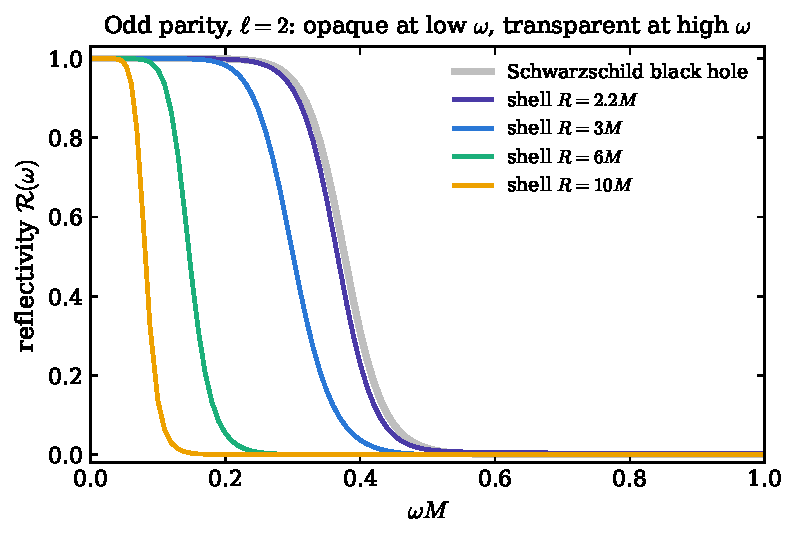
\includegraphics[width=\linewidth]{r3_f02_reflectivity_odd.pdf}
\caption{Odd-parity reflectivity, $\ell=2$, for four compactnesses, and the black hole.}\label{fig:R}\end{minipage}\hfill
\begin{minipage}{0.49\textwidth}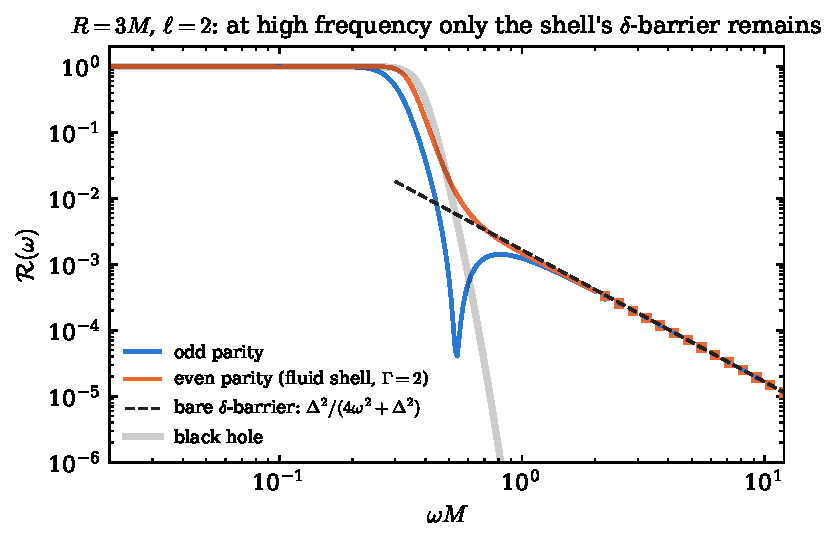
\includegraphics[width=\linewidth]{r3_f03_highfreq_law.pdf}
\caption{Log--log view at $R=3M$: both parities follow the $\delta$-barrier law at high frequency.}\label{fig:hf}\end{minipage}
\\[4mm]
\begin{minipage}{0.49\textwidth}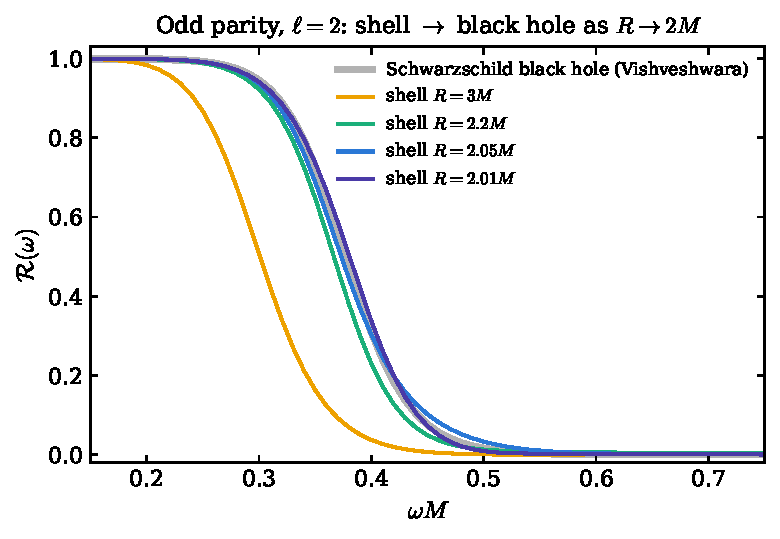
\includegraphics[width=\linewidth]{r3_f04_bh_limit.pdf}
\caption{Approach to the black-hole reflectivity as $R\to2M$ (odd, $\ell=2$).}\label{fig:bh}\end{minipage}\hfill
\begin{minipage}{0.49\textwidth}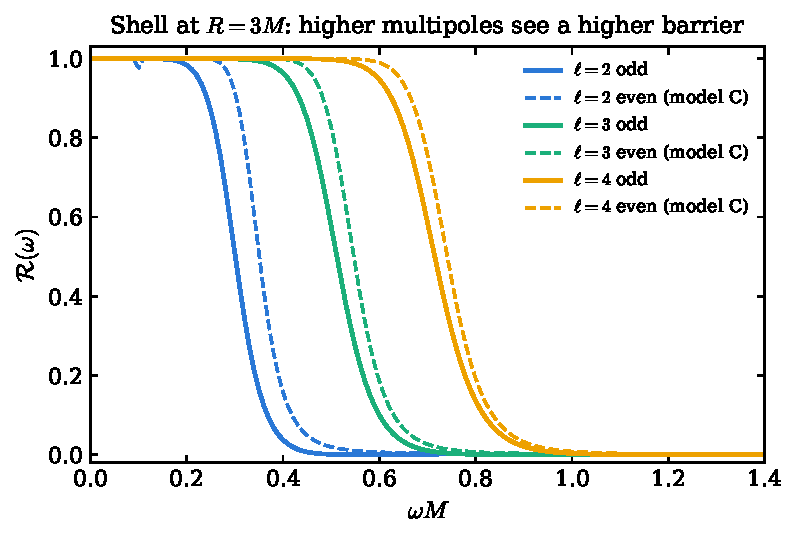
\includegraphics[width=\linewidth]{r3_f13_multipoles.pdf}
\caption{$\ell=2,3,4$ at $R=3M$. Solid: odd; dashed: even (model C, $\Gamma=2$).}\label{fig:ell}\end{minipage}
\\[4mm]
\begin{minipage}{0.49\textwidth}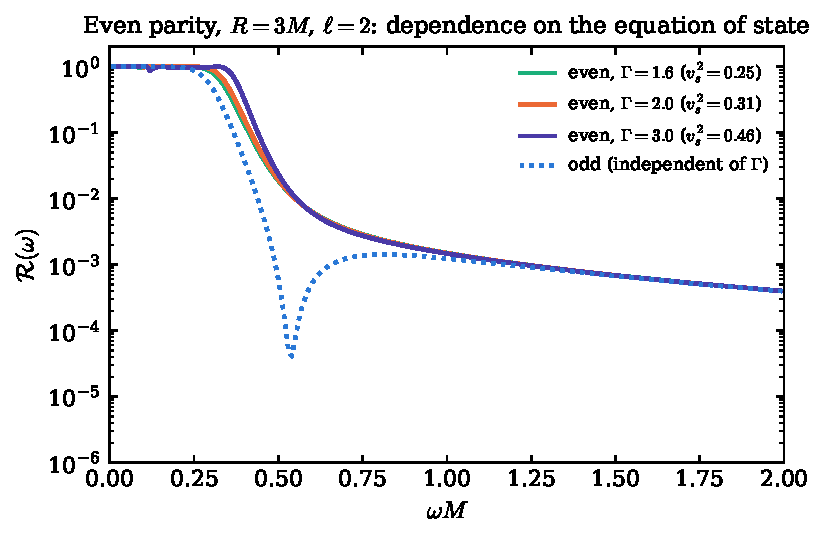
\includegraphics[width=\linewidth]{r3_f14_eos.pdf}
\caption{Even parity at $R=3M$ for three adiabatic indices. The narrow features at low $\omega$ are matter resonances.}\label{fig:eos}\end{minipage}\hfill
\begin{minipage}{0.49\textwidth}\centering\small
\captionof{table}{Approach to the black-hole reflectivity ($\ell=2$; even: model C).}\label{tab:bhlimit}
\setlength{\tabcolsep}{3pt}
\begin{tabular}{rrrrr}\toprule
$\omega M$ & BH & odd $2.2M$ & odd $2.05M$ & odd $2.002M$\\\midrule
0.30 & 0.94521 & 0.92247 & 0.93661 & 0.94729\\
0.37 & 0.56378 & 0.46896 & 0.52601 & 0.56105\\
0.45 & 0.07559 & 0.04894 & 0.10167 & 0.07539\\
0.60 & 0.00066 & 0.00554 & 0.00319 & 0.00021\\\bottomrule
\end{tabular}
\end{minipage}
\end{figure}

\begin{learned}
The shell is opaque to long waves, transparent to short ones ($\RR\propto\Delta^2/\omega^2$), and black-hole-like when very
compact. Parity and equation of state matter only at intermediate frequencies.
\end{learned}

%==========================================================================================
\section{Step 5 --- Numerical methods and why we trust them}\label{sec:num}
\begin{question}
The coefficients and the QNMs need the exterior solutions for arbitrary complex $\omega$. How do we compute them
reliably, and how do we test the result?
\end{question}
\paragraph{Method 1: transfer matrix with a continued-fraction exterior.} The outgoing exterior solution is expanded as
$\Psi_{\rm up}=(r-2M)^{2iM\omega}e^{i\omega r}\sum_na_n(1-R_2/r)^n$ about a point $R_2\ge4M$
\cite{LNS93,Pani09}. The coefficients satisfy a four-term recurrence. It is reduced to three terms by Gaussian
elimination \cite{Leaver90}, and the minimal solution is selected by a continued fraction \cite{Gautschi67}. This gives
$\Psi_{\rm up}'/\Psi_{\rm up}$ to $10^{-12}$ for any complex $\omega$. Zerilli solutions follow from the Chandrasekhar map.
The interior solution is pushed through $\mathsf T$ and decomposed into in/up waves at $R$.
\paragraph{Method 2: shooting.} The equation is integrated from $R$ outward to $r_{\rm far}=\max(150M,60/\omega)$ with DOP853
\cite{Hairer93,SciPy20} (rtol $10^{-10}$), and the solution is projected on high-order asymptotic series. For QNMs we
integrate \emph{inward} from a far point on a complex ray where the outgoing solution is subdominant, following
Boyanov et al.\ \cite{Boyanov25}. The two methods share only the junction matrix and the interior functions.
\paragraph{QNMs.} They are zeros of the Wronskian between the solution coming from the regular interior through the
junction and the outgoing solution. Candidates come from scans of $\log|W|$ in the complex plane and are refined by
Newton iteration. Every root is re-converged with the other method.
\paragraph{Black-hole benchmarks and WKB.} Black-hole QNMs come from Leaver's continued fraction \cite{Leaver85}. WKB
estimates of orders 1, 3 and 6 \cite{SW85,IW87,Iyer87,Konoplya03} are computed with an arbitrary-order recursion
\cite{Hatsuda20,BenderWu69,Killingbeck78,FernandezCastro87}. For trapped modes we use a Bohr--Sommerfeld condition with
Langer's correction \cite{Langer37} plus Gamow tunnelling.

\begin{table}[h]\centering\small
\caption{Validation summary.}\label{tab:valid}
\begin{tabular}{ll}\toprule
test & result\\\midrule
energy balance $|\RR+\TT-1|$, odd and even (model C), $\omega M\in[0.005,2]$ & $\le6\times10^{-10}$\\
Method 1 vs Method 2 on $\RR,\TT$ & $\lesssim10^{-9}$\\
Method 1 vs Method 2 on 397 QNMs & median $4\times10^{-12}$, worst $6\times10^{-5}$\\
low frequency $1-\RR$ at $\omega M=10^{-3}$ & $<10^{-15}$\\
$\det\mathsf T\sq-1$ (even, model C) & $\le10^{-12}$\\
Schwarzschild $\ell=2,n=0$ (Leaver) & $0.3736716844-0.0889623157i$, as in \cite{BCS09}\\
black-hole reflectivity at $(2M\omega)^2=1$, $4$ & $1.55\times10^{-2}$, $5.3\times10^{-9}$ \cite{Vishveshwara70}\\
RW vs Zerilli black-hole reflectivity (isospectrality) & equal to $10^{-7}$\\
WKB relative error, $\ell=2,n=0$, orders 1/3/6 & $6.6\times10^{-2}$ / $1.5\times10^{-3}$ / $2.3\times10^{-4}$\\
time-domain ringdown vs QNM (Sec.~\ref{sec:td}) & agreement to $\sim10^{-3}$\\\bottomrule
\end{tabular}
\end{table}

\begin{figure}[h]\centering
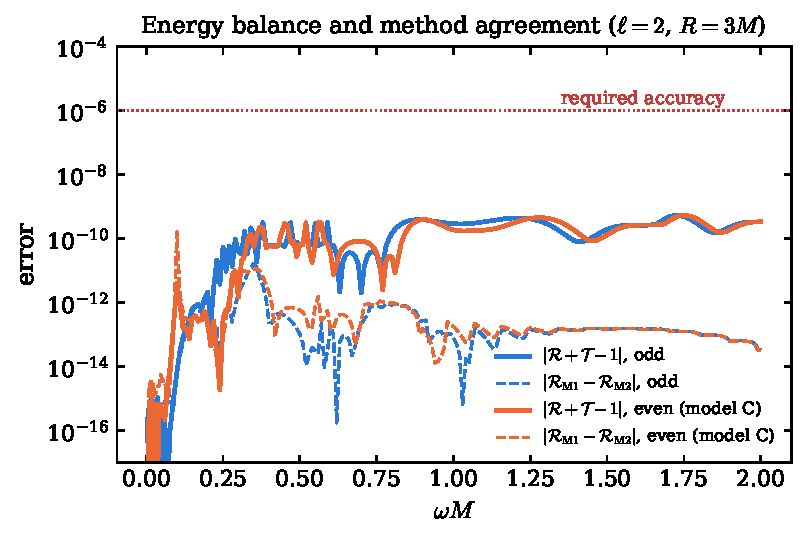
\includegraphics[width=0.62\textwidth]{r3_f08_validation.pdf}
\caption{Energy balance (solid) and agreement between the two methods (dashed) at $R=3M$, $\ell=2$.}\label{fig:valid}
\end{figure}

\begin{table}[h]\centering\small
\caption{Schwarzschild QNMs $\omega M$: Leaver's continued fraction vs WKB of orders 1, 3 and 6.}\label{tab:bhqnm}
\begin{tabular}{rrllll}\toprule
$\ell$ & $n$ & Leaver CF (this code) & WKB 1st & WKB 3rd & WKB 6th\\\midrule
2 & 0 & $0.37367168-0.08896232i$ & $0.3988-0.0883i$ & $0.37316-0.08922i$ & $0.373619-0.088891i$ \\
2 & 1 & $0.34671100-0.27391488i$ & $0.4534-0.2330i$ & $0.34602-0.27492i$ & $0.346297-0.273480i$ \\
2 & 2 & $0.30105345-0.47827698i$ & $0.5170-0.3406i$ & $0.30293-0.47106i$ & $0.298520-0.477560i$ \\
2 & 3 & $0.25150496-0.70514820i$ & $0.5775-0.4268i$ & $0.24746-0.67290i$ & $0.241715-0.709595i$ \\
3 & 0 & $0.59944329-0.09270305i$ & $0.6166-0.0923i$ & $0.59927-0.09273i$ & $0.599443-0.092703i$ \\
3 & 1 & $0.58264380-0.28129811i$ & $0.6619-0.2580i$ & $0.58235-0.28141i$ & $0.582642-0.281290i$ \\
3 & 2 & $0.55168490-0.47909275i$ & $0.7251-0.3925i$ & $0.55320-0.47668i$ & $0.551594-0.479047i$ \\
3 & 3 & $0.51196191-0.69033710i$ & $0.7909-0.5038i$ & $0.51575-0.67743i$ & $0.511099-0.690468i$ \\
4 & 0 & $0.80917838-0.09416396i$ & $0.8223-0.0939i$ & $0.80910-0.09417i$ & $0.809178-0.094164i$ \\
4 & 1 & $0.79663153-0.28433435i$ & $0.8602-0.2694i$ & $0.79650-0.28437i$ & $0.796631-0.284334i$ \\
4 & 2 & $0.77270953-0.47990818i$ & $0.9187-0.4204i$ & $0.77364-0.47897i$ & $0.772695-0.479900i$ \\
4 & 3 & $0.73983673-0.68392432i$ & $0.9844-0.5492i$ & $0.74331-0.67830i$ & $0.739665-0.683902i$ \\
\bottomrule\end{tabular}

\end{table}

%==========================================================================================
\section{Step 6 --- How the shell rings: quasinormal modes}\label{sec:qnm}
\begin{question}
A black hole rings at $0.3737-0.0890i$ ($\ell=2$). What are the characteristic frequencies of the shell, and do they
approach the black-hole ones when $R\to2M$?
\end{question}
QNMs are the complex frequencies at which the regular interior solution, continued through the shell, is purely outgoing
at infinity. Physically, they are the free oscillations of the object. We find three families.

\paragraph{1. Wave (cavity) modes.} The flat interior is a resonant cavity whose ``walls'' are the shell and the
exterior barrier. For dilute shells PSP26 derived ${\rm Re}(\omega R)\simeq n\pi$ or $(n+\tfrac12)\pi$ and
${\rm Im}(\omega R)\simeq-\xi$, with $\xi=\tfrac12\ln[2\ell(\ell+1)R/M]$ (their Eqs.~7.23--7.25). The cavity leaks through a
weakly reflecting wall, so the damping is strong and grows only logarithmically with $R/M$. Our wave modes agree with
PSP26 (Table~\ref{tab:psp}).

\paragraph{2. Trapped modes ($R<3M$).} When the shell is inside the photon sphere, waves with $\omega^2<V_{\max}$ are
trapped between the interior centrifugal barrier and the exterior barrier. They leak out only by tunnelling. Their
damping becomes exponentially small as $R\to2M$ (Table~\ref{tab:trapped}), and a WKB Bohr--Sommerfeld estimate reproduces
their real parts to a few per cent. These long-lived modes produce gravitational-wave \emph{echoes}
\cite{Cardoso2016PRL,Abedi2017}.

\paragraph{3. Matter modes} (even parity, model C). These are oscillations of the shell's own fluid, with
$\omega\sim(M/R^3)^{1/2}$ (Sec.~\ref{sec:matter}).

\begin{keyidea}
None of the shell modes tends to a Schwarzschild QNM as $R\to2M$ (Fig.~\ref{fig:qnm}). The reflectivity is continuous in
the black-hole limit, but the spectrum is not. The black hole's ringing comes from waves at the photon sphere leaking
\emph{inward}, into the horizon. A shell reflects those waves back and replaces the black-hole modes by trapped modes.
\end{keyidea}

\begin{figure}[t]\centering
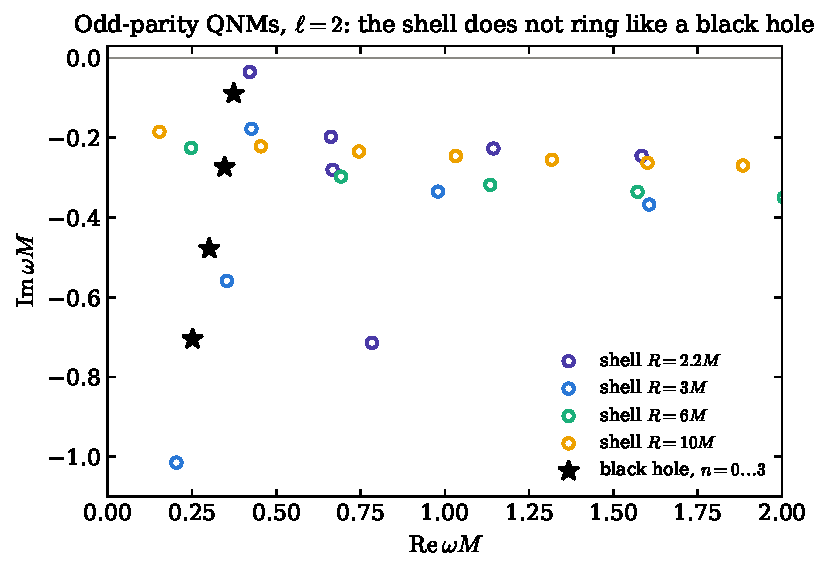
\includegraphics[width=0.66\textwidth]{r3_f05_qnm_plane.pdf}
\caption{Odd-parity QNMs ($\ell=2$) in the complex plane for four compactnesses (circles), and the Schwarzschild
overtones (stars). At $R=2.2M$ the least-damped mode sits close to the real axis: it is a trapped mode.}\label{fig:qnm}
\end{figure}

\begin{table}[h]\centering\small
\caption{Wave modes ($\ell=2$; even: model C, $\Gamma=2$) compared with PSP26 Figs.~3--4 (reading uncertainty $\pm0.02$).}\label{tab:psp}
\begin{tabular}{lrrrrrr}\toprule
parity & $M/R$ & mode & ${\rm Re}(R\omega)$ & ${\rm Im}(R\omega)/\xi$ & PSP26 Re & PSP26 Im$/\xi$\\\midrule
odd & 0.167 & 1 & 1.484 & -0.632 & 1.47 & -0.630 \\
odd & 0.167 & 2 & 4.151 & -0.835 & 4.10 & -0.840 \\
even & 0.250 & 1 & 1.033 & -0.651 & 1.05 & -0.655 \\
even & 0.100 & 1 & 0.615 & -0.825 & 0.62 & -0.825 \\
even & 0.100 & 2 & 2.978 & -0.907 & 2.95 & -0.910 \\
\bottomrule\end{tabular}

\end{table}
\begin{table}[h]\centering\small
\caption{Trapped modes of ultracompact shells (odd, $\ell=2$): exact vs WKB.}\label{tab:trapped}
\begin{tabular}{rll}\toprule
$R/M$ & exact (M1) & WKB (Bohr--Sommerfeld + Gamow)\\\midrule
2.01 & $0.162603-9.711e-07\,i$ & $0.152432-5.081e-07\,i$ \\
2.01 & $0.248683-5.284e-05\,i$ & $0.246194-3.249e-05\,i$ \\
2.01 & $0.326133-8.798e-04\,i$ & $0.328792-7.287e-04\,i$ \\
2.02 & $0.216610-1.809e-05\,i$ & $0.205905-8.922e-06\,i$ \\
2.02 & $0.322125-1.072e-03\,i$ & $0.324183-8.289e-04\,i$ \\
2.05 & $0.302815-8.384e-04\,i$ & $0.296095-4.811e-04\,i$ \\
2.10 & $0.367989-8.195e-03\,i$ & $0.370495-7.304e-03\,i$ \\
\bottomrule\end{tabular}

\end{table}
\begin{table}[h]\centering\scriptsize
\caption{Lowest QNMs, $\ell=2$ (the even-A rows refer to the frozen wall and should be read with the caveat of
Sec.~\ref{sec:backto1}). The stable matter pair at $R=2.2M$ and $3M$, $0.18592-0.00003i$ and $0.19712-0.00031i$, is not
listed.}\label{tab:qnm2}
\begin{tabular}{rlp{12cm}}\toprule
$R/M$ & sector & lowest wave modes $\omega M$ (ordered by ${\rm Re}\,\omega$; Methods 1 and 2 agree to $<10^{-4}$)\\\midrule
2.2 & odd & $0.42111-0.03502i$, $0.66196-0.19736i$, $0.66692-0.28043i$, $0.78377-0.71437i$ \\
2.2 & even-C & $0.44694-0.04385i$, $0.57996-0.19970i$, $0.69756-0.56050i$, $0.92055-0.21412i$; matter: $0.00000+0.24429i$, $0.00000-0.24429i$ \\
2.2 & even-A & $0.10284-0.04070i$, $0.45445-0.10428i$, $0.56024-0.44388i$, $0.65595-0.85878i$ \\
3 & odd & $0.20371-1.01489i$, $0.35352-0.55904i$, $0.42638-0.17728i$, $0.97955-0.33508i$ \\
3 & even-C & $0.21102-0.76599i$, $0.40766-0.29425i$, $0.61594-0.31862i$, $1.91546-0.38053i$; matter: $-0.00000+0.13321i$, $-0.00000-0.13326i$ \\
3 & even-A & $0.05288-0.97817i$, $0.24913-0.59916i$, $0.35675-0.22995i$, $0.96224-0.13441i$ \\
6 & odd & $0.24739-0.22534i$, $0.69189-0.29749i$, $1.13482-0.31819i$, $1.57166-0.33553i$ \\
6 & even-C & $0.13710-0.26885i$, $0.45011-0.28793i$, $0.91288-0.30736i$, $1.35361-0.32702i$; matter: $0.08942-0.00005i$, $-0.00000+0.04014i$, $-0.00000-0.04014i$ \\
6 & even-A & $0.18120-0.22393i$, $0.66401-0.17021i$, $1.12337-0.19838i$, $1.56453-0.21844i$ \\
10 & odd & $0.15342-0.18490i$, $0.45405-0.22153i$, $0.74518-0.23457i$, $1.03239-0.24567i$ \\
10 & even-C & $0.06152-0.19748i$, $0.29784-0.21714i$, $0.59930-0.22783i$, $0.88902-0.24022i$; matter: $0.04421-0.00001i$, $-0.00000+0.01762i$, $0.00000-0.01762i$ \\
10 & even-A & $0.11383-0.17403i$, $0.43293-0.14212i$, $0.73603-0.15791i$, $1.02659-0.17041i$ \\
\bottomrule\end{tabular}

\end{table}

\subsection{Seeing the modes in the time domain}\label{sec:td}
The QNMs can also be seen directly. We solved $\partial_t^2\Psi=\partial_x^2\Psi-V(x)\Psi-\Delta\,\delta(x-x_R)\Psi$ (odd,
$\ell=2$) with a leapfrog scheme in the global coordinate~\eqref{eq:x}. The centre was regular and the outer boundary
absorbing; for the black hole we used an absorbing boundary deep in the throat. The same Gaussian pulse (width $3M$)
was sent onto each object and recorded at $x=75M$ (Fig.~\ref{fig:td}).
\begin{itemize}
\item \emph{Black hole}: a short ringdown. A fit gives $\omega M=0.3731-0.0885i$, against Leaver's $0.3737-0.0890i$.
\item \emph{Shell at $R=2.2M$}: after the prompt reflection the signal keeps ringing for hundreds of $M$. The fit gives
$0.4215-0.0352i$, against the frequency-domain trapped mode $0.4211-0.0350i$.
\item \emph{Shell at $R=3M$}: the cavity modes are strongly damped, and the signal soon joins the late-time power-law tail
of the Schwarzschild exterior, which is common to all three objects.
\end{itemize}
This is a fully independent check of the frequency-domain spectrum, since it shares no code with it.

\begin{figure}[t]\centering
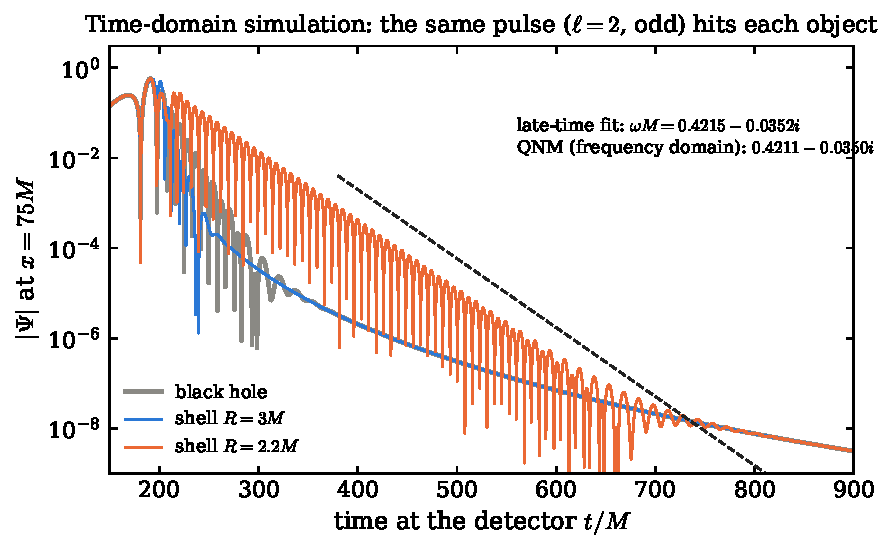
\includegraphics[width=0.49\textwidth]{r3_f11_timedomain.pdf}\hfill
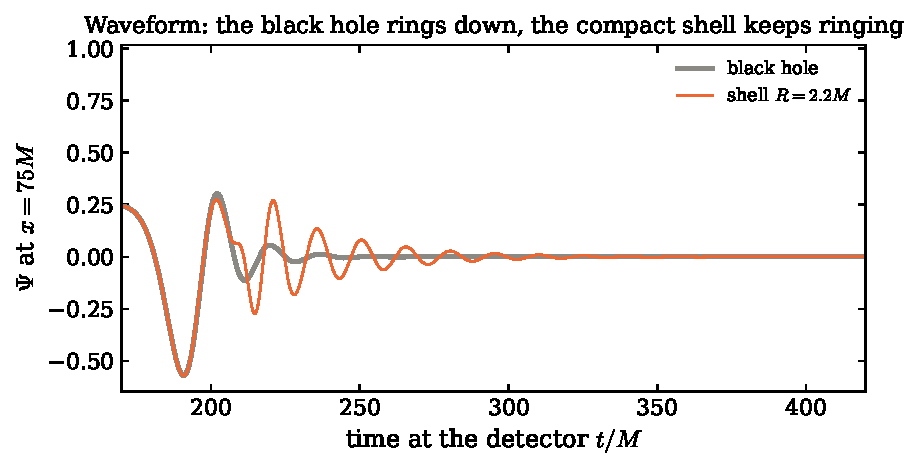
\includegraphics[width=0.49\textwidth]{r3_f12_waveform.pdf}
\caption{Time-domain simulation. Left: $|\Psi|$ at the detector (log scale); the dashed line is the decay rate of the
trapped QNM. Right: the waveform, with the black hole ringing down and the compact shell continuing to ring.}\label{fig:td}
\end{figure}

\begin{learned}
The shell rings through cavity modes, long-lived trapped modes (for $R<3M$) and matter modes. The black-hole QNMs are
\emph{not} a limit of this spectrum, although the black-hole reflectivity is a limit of $\RR(\omega)$.
\end{learned}

%==========================================================================================
\section{Step 7 --- Is the static shell stable? The matter modes}\label{sec:matter}
\begin{question}
Model C was chosen because it is static. If one of its modes has ${\rm Im}\,\omega>0$, it is unstable. Is it?
\end{question}
In the even sector we find four matter modes per $\ell$: a purely imaginary growing mode, its damped mirror, and a pair
$\pm{\rm Re}\,\omega+i\,{\rm Im}\,\omega$ with small negative imaginary part. At $M/R=0.2$, $\ell=2$, $\Gamma=2$:
\begin{equation}
\omega\,(R^3/M)^{1/2}=0.6077\,i\quad(\text{growing}),\qquad 1.2671-0.0011\,i\quad(\text{oscillating}).
\end{equation}
\textbf{The static fluid shell is linearly unstable}, with $e$-folding time $\simeq1.6(R^3/M)^{1/2}$. An unstable mode was
found for every $\ell$ and $R$ examined.

\paragraph{Comparison with PSP26.} PSP26 use a different formalism: retarded-time slicing, a RW-type master function in both
sectors, and spectral or MST-type solvers. Reproducing their numbers therefore tests our even junction independently.
The agreement holds at all compactnesses (Table~\ref{tab:pitre}, Fig.~\ref{fig:matter}) and for the dependence on
$\Gamma$ in their Figs.~1--2.

\paragraph{Where does the instability come from? A Newtonian picture.} As $M/R\to0$ the frequencies tend to those of a
\emph{Newtonian} self-gravitating 2D fluid shell, which can be derived in half a page (App.~\ref{app:newton}). Equilibrium
requires $p=\sigma M/4R$, the Newtonian limit of Eq.~\eqref{eq:kappa}. For deformations
$\propto Y_{\ell m}e^{-i\omega t}$ one finds $\varsigma^4-S\varsigma^2+P=0$ with $\varsigma^2=\omega^2R^3/M$ and
\begin{equation}
S=\frac{(\ell^2+\ell+4)\Gamma-(\ell^2+\ell+6)}{4},\qquad
P=-\frac{(\ell-1)\ell(\ell+1)\big[(\ell+2)(2\ell-3)\Gamma-4(\ell-2)\big]}{16(2\ell+1)} .
\end{equation}
For $\ell\ge2$ and the relevant $\Gamma$, $P<0$, so one root $\varsigma^2$ is negative: a purely imaginary, growing mode. For
$\ell=2$, $\Gamma=2$ the roots are $\varsigma=1.5050$ and $0.5147\,i$, the $M/R\to0$ end points of Fig.~\ref{fig:matter}.
\begin{keyidea}
The shell is held up by \emph{tangential} pressure against its own gravity. A non-spherical deformation changes the
curvature and the density in such a way that the restoring force is outweighed: the membrane buckles. This is ordinary
Newtonian physics; general relativity only shifts the numbers by $O(M/R)$.
\end{keyidea}
The same derivation reproduces PSP26's closed-form Eq.~(7.8) identically. It also shows that the constant term of their
quartic, Eq.~(7.6), contains a misprint: as printed, $(\ell+2)[(2\ell-3)\Gamma-4]$ would predict stability for $\ell=2$.

\begin{figure}[t]\centering
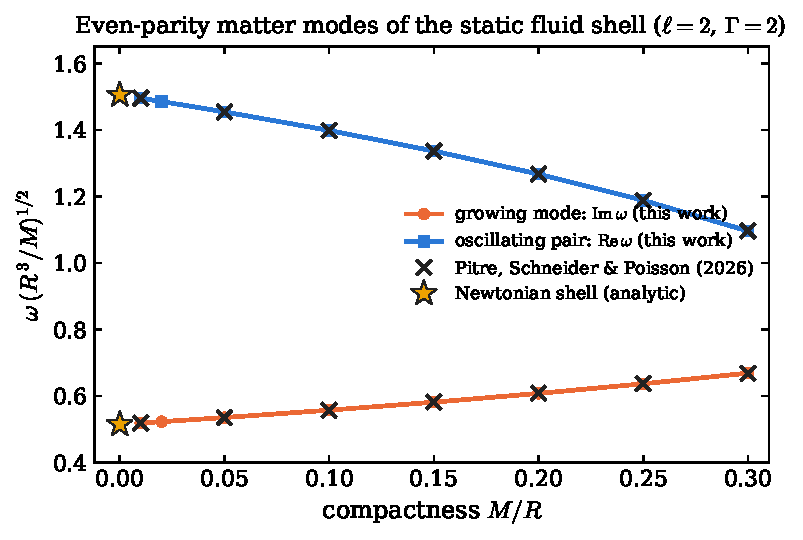
\includegraphics[width=0.66\textwidth]{r3_f06_matter_modes.pdf}
\caption{Matter modes vs compactness ($\ell=2$, $\Gamma=2$): growing mode (${\rm Im}\,\omega$, orange) and oscillating pair
(${\rm Re}\,\omega$, blue). Crosses: values read from PSP26. Stars: Newtonian shell.}\label{fig:matter}
\end{figure}
\begin{table}[h]\centering\small
\caption{Matter modes of the fluid shell, $\ell=2$, $\Gamma=2$ ($|\Delta_{12}|$: difference between the two methods).}\label{tab:pitre}
\begin{tabular}{rllll}\toprule
$M/R$ & unstable: $\omega(R^3/M)^{1/2}$ & $|\Delta_{12}|$ & stable pair: $\omega(R^3/M)^{1/2}$ & $|\Delta_{12}|$\\\midrule
0.30 & $0.668693\,i$ & 1.6e-12 & $1.095903-1.70e-03\,i$ & 1.8e-12 \\
0.25 & $0.636634\,i$ & 7.1e-12 & $1.188088-1.51e-03\,i$ & 9.2e-13 \\
0.20 & $0.607709\,i$ & 1.6e-11 & $1.267067-1.10e-03\,i$ & 3.9e-13 \\
0.15 & $0.581398\,i$ & 2.3e-11 & $1.336362-6.47e-04\,i$ & 5.1e-13 \\
0.10 & $0.557313\,i$ & 3.3e-11 & $1.398197-2.78e-04\,i$ & 6.1e-13 \\
0.05 & $0.535158\,i$ & 4.6e-11 & $1.454057-5.79e-05\,i$ & 7.4e-13 \\
0.02 & $0.522690\,i$ & 4.6e-11 & $1.485144-6.52e-06\,i$ & 8.3e-13 \\
0.01 & $0.518662\,i$ & 6.1e-11 & $1.495140-1.20e-06\,i$ & 0.0e+00 \\
$\to0$ (PN, PSP26 Eq.~7.8) & $0.514695\,i$ & & $1.504962$ & \\
\bottomrule\end{tabular}

\end{table}

\begin{learned}
The only static member of the family is unstable, as PSP26 found. The instability is Newtonian in origin and grows on
the slow time scale $(R^3/M)^{1/2}$.
\end{learned}

%==========================================================================================
\section{Step 8 --- Back to the background: are the models consistent?}\label{sec:backto1}
\begin{question}
Every frequency-domain result assumes a background that does not change during a wave period. Neither model is
eternally static. When is the idealization justified?
\end{question}
\begin{keyidea}
Compare three rates: the wave frequencies ($|\omega|\sim1/R$), the growth rate of the fluid shell's instability, and
the collapse rate of the domain wall (Fig.~\ref{fig:time}).
\end{keyidea}
\paragraph{Fluid shell (model C): justified.} The instability grows at $\simeq0.6(M/R^3)^{1/2}$, a factor
$\sim(R/M)^{1/2}$ slower than the waves. Many wave periods fit into one $e$-folding, so scattering and ringing off model C
are meaningful adiabatic idealizations for $\omega(R^3/M)^{1/2}\gg1$.

\paragraph{Domain wall (model A): not justified.} From Eq.~\eqref{eq:Rdd}, $\omega_{\rm dyn}=\sq(|\ddot R|/R)^{1/2}\to\sqrt2/R$
for large $R$. A tension-driven wall collapses on the \emph{light-crossing time}, whatever $M$ is, and that time is
comparable to the wave periods. The frozen snapshot is therefore at best marginal. The junction conditions show the
problem explicitly:
\begin{itemize}
\item In the odd sector the frozen system is consistent (4 equations, rank 3), and the result is identical to model C's
$\delta$-barrier. \emph{Odd-parity results hold for both models.}
\item In the even sector the frozen, monochromatic ansatz is not a solution of the moving-shell problem. The system has
8 equations for 6 unknowns, with ${\rm rank}\,\mathsf A=6$ but ${\rm rank}[\mathsf A|\mathsf B]=8$: it is
\emph{inconsistent}. One must choose which two of the four Israel equations to drop. Different, equally defensible
choices give reflectivities that differ at $O(1)$ even at $\omega M=30$, from total reflection down to the
$\delta$-law (Fig.~\ref{fig:modelA}), and QNMs that differ by 20--30\%. Keeping the two angular equations leads to
an energy error larger than $\RR$ itself. Only the choice ``$\tau\tau$ + trace-free'' conserves energy and reproduces the
universal high-frequency law.
\end{itemize}
\textbf{Conclusion:} the even-parity scattering and QNMs of a frozen domain wall are \emph{not} determined by the
freezing approximation. A trustworthy answer would need a genuinely time-dependent treatment of the collapsing wall.

\begin{figure}[t]\centering
\begin{minipage}{0.49\textwidth}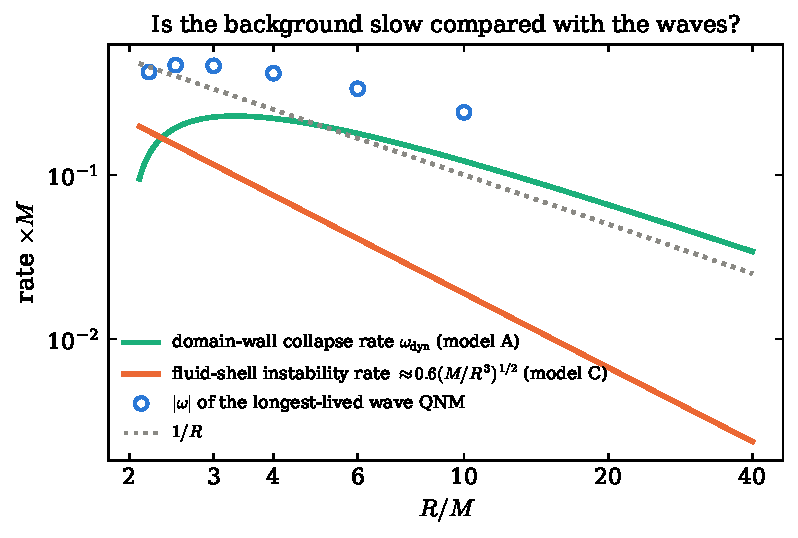
\includegraphics[width=\linewidth]{r3_f07_timescales.pdf}
\caption{Rates as functions of $R/M$. The wall collapses as fast as the waves oscillate; the fluid instability is
slow.}\label{fig:time}\end{minipage}\hfill
\begin{minipage}{0.49\textwidth}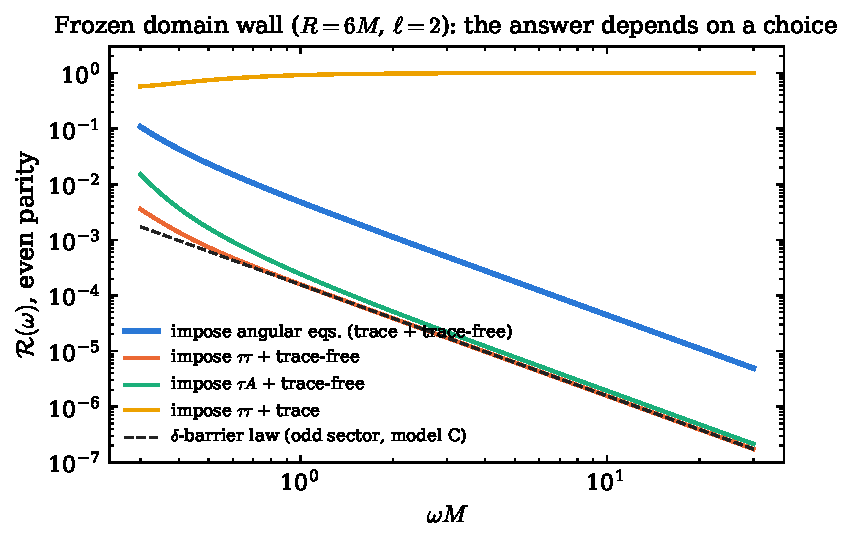
\includegraphics[width=\linewidth]{r3_f10_modelA_ambiguity.pdf}
\caption{Frozen wall, even parity, $R=6M$: the reflectivity depends on which Israel equations are imposed.}\label{fig:modelA}\end{minipage}
\end{figure}

\begin{learned}
The static fluid shell is a sound model for scattering and ringing even though it is unstable, because the
instability is slow. The frozen domain wall is not a controlled approximation for even parity; its odd sector coincides
with model C's.
\end{learned}

%==========================================================================================
\section{Summary and outlook}\label{sec:concl}
\paragraph{Answers to the eight questions.}
\begin{enumerate}
\item A static thin shell with flat interior needs positive surface pressure, $p/\sigma=(1-\sq)/4\sq$. Domain walls and
dust collapse.
\item Waves obey the RW/Zerilli equations outside and the flat equation inside, with interior frequency $\nu=\omega/\sq$.
\item Odd parity: $[\Psi]=0$ and $[\partial_x\Psi]=\Delta\Psi$ with $\Delta=\sq(1-\sq)/R$. Even parity: a flux-conserving $2\times2$
matrix, with $\det\mathsf T=f_R^{-1/2}$.
\item $\RR\to1$ as $\omega\to0$; $\RR\simeq\Delta^2/4\omega^2$ as $\omega\to\infty$; $\RR\to\RR_{\rm BH}$ as $R\to2M$.
\item Two methods agree to $10^{-9}$ (scattering) and $\le6\times10^{-5}$ (QNMs), and all limits and benchmarks are
reproduced.
\item The QNMs are cavity modes, trapped (echo) modes and matter modes. The black-hole spectrum is not their limit. A
time-domain simulation confirms them.
\item The static shell is unstable, through a Newtonian buckling mode; this agrees with PSP26.
\item The fluid shell is a valid adiabatic model; the frozen wall is not, for even parity.
\end{enumerate}
\paragraph{New results.} The reflection and transmission coefficients and their limits; the explicit $\delta$-function
form of the odd junction and its thick-shell derivation; the assessment of the frozen domain wall; the Newtonian
derivation and the misprint in PSP26 (7.6).
\paragraph{Limitations and outlook.} Model C is restricted to $R\ge25M/12$ by the energy and causality conditions. The
open-interior definition of $\RR$ and $\TT$ is a convention adapted to the question ``how much does the object send
back''; for the closed system $|S|=1$. Natural next steps are a time-domain evolution of the unstable shell into the
nonlinear regime, a de Sitter interior (gravastar), and a time-dependent treatment of the collapsing domain wall.

%==========================================================================================
\appendix
\section{Newtonian oscillations of a self-gravitating fluid shell}\label{app:newton}
Take a shell of radius $R$, surface density $\sigma$, 2D pressure $p$ and mass $M=4\pi R^2\sigma$ ($G=1$). The field acting
on the shell is the average of the interior (zero) and exterior ($-M/R^2$) fields. The normal force of a 2D fluid of
pressure $p$ on a surface of mean curvature $2H$ is $2Hp$, outward. Equilibrium therefore requires
$2p/R=\sigma M/2R^2$, i.e.\ $p=\sigma M/4R$, the Newtonian limit of Eq.~\eqref{eq:kappa}. Let the displacement be
$\xi_rY\hat r+\xi_h\nabla_{S^2}Y$ with time dependence $e^{-i\omega t}$, and define $x=\xi_r/R$ and $y=\xi_h/R$. Then:
\begin{itemize}
\item continuity: $\Delta\sigma/\sigma=-(2x-\lambda y)$ with $\lambda=\ell(\ell+1)$, and $\Delta p=\Gamma p\,\Delta\sigma/\sigma$;
\item self-gravity: the displaced sheet acts on the exterior like a surface density $\sigma(\lambda y+\ell x)Y$ and on the
interior like $\sigma(\lambda y-(\ell+1)x)Y$;
\item mean curvature: $2H=2/R-(2-\lambda)xY/R$.
\end{itemize}
With $\varsigma^2=\omega^2R^3/M$ the radial and tangential equations of motion are
\begin{align}
\varsigma^2x&=-x+\frac{\lambda(y+2x)}{2(2\ell+1)}+\frac\Gamma2(2x-\lambda y)+\frac{(2-\lambda)x}{4}-\frac{2x-\lambda y}{2},\\
\varsigma^2y&=-\frac\Gamma4(2x-\lambda y)-\frac{\lambda y-(\ell+1)x}{2\ell+1}.
\end{align}
The trace and determinant of this $2\times2$ problem give $S$ and $P$ of Sec.~\ref{sec:matter}. The roots coincide
identically with PSP26's Eq.~(7.8).

\section{Axial perturbations of an anisotropic fluid and the thin-shell limit}\label{app:axial}
For $\dd s^2=-e^{2\Phi}\dd t^2+e^{2\Lambda}\dd r^2+r^2\dd\Omega^2$, with $e^{-2\Lambda}=1-2m/r$ and
$T_{\mu\nu}=(\rho+p_t)u_\mu u_\nu+p_tg_{\mu\nu}+(p_r-p_t)s_\mu s_\nu$, consider an axial perturbation $h_0,h_1$ (RW gauge)
and $\delta u_\phi$. With $X=e^{\Phi-\Lambda}h_1/r$ and $\dd r_*=e^{\Lambda-\Phi}\dd r$,
\begin{equation}
X_{,r_*r_*}+\big\{\omega^2-e^{2\Phi}[\ell(\ell+1)/r^2-6m/r^3+4\pi(\rho-p_r)]\big\}X=0,
\end{equation}
once $m'=4\pi r^2\rho$, $\Phi'=(m+4\pi r^3p_r)/r(r-2m)$ and the anisotropic TOV equation are used. For $p_r=0$ and a layer
whose thickness tends to zero, $\int\rho\,\dd\ell_{\rm p}=(1-\sq)/4\pi R=\sigma$ and $\int p_t\,\dd\ell_{\rm p}=p$: exactly
the model-C background. The only singular term of the potential is $4\pi\rho e^{2\Phi}\to\Delta\,\delta(x-x_R)$ with
$\Delta=4\pi\sigma\sq$. This is Eq.~\eqref{eq:odd}.

\section{Code and reproducibility}
\begin{tabular}{p{6.2cm}p{8.6cm}}\toprule
\texttt{First round/code/} & derivation and numerics: symbolic junction conditions (\texttt{symbolic/}), background,
interior, exterior, scattering, QNMs, WKB (\texttt{shellgw/}); driver \texttt{main.py}\\
\texttt{First round/results/} & scattering curves, QNM catalogue, validation data (JSON/CSV)\\
\texttt{Second round/checks/} & independent solver, thick-shell test, Newtonian shell, model-A analysis\\
\texttt{Third round/code/make\_figures\_r3.py} & all figures of this paper, the high-frequency points and the
time-domain simulation (\texttt{python -B make\_figures\_r3.py})\\\bottomrule
\end{tabular}

%==========================================================================================
\begin{thebibliography}{99}\small
\bibitem{RW57} T.~Regge and J.~A.~Wheeler, Stability of a Schwarzschild singularity, Phys.\ Rev.\ \textbf{108}, 1063 (1957).
\bibitem{Zerilli70} F.~J.~Zerilli, Effective potential for even-parity Regge--Wheeler gravitational perturbation equations, Phys.\ Rev.\ Lett.\ \textbf{24}, 737 (1970).
\bibitem{Vishveshwara70} C.~V.~Vishveshwara, Scattering of gravitational radiation by a Schwarzschild black-hole, Nature \textbf{227}, 936 (1970).
\bibitem{MP05} K.~Martel and E.~Poisson, Gravitational perturbations of the Schwarzschild spacetime: a practical covariant and gauge-invariant formalism, Phys.\ Rev.\ D \textbf{71}, 104003 (2005); K.~Martel, PhD thesis, University of Guelph (2004).
\bibitem{IS84} J.~Ipser and P.~Sikivie, Gravitationally repulsive domain wall, Phys.\ Rev.\ D \textbf{30}, 712 (1984).
\bibitem{Poisson04} E.~Poisson, \emph{A Relativist's Toolkit} (Cambridge University Press, 2004), Ch.~3.
\bibitem{AS72} M.~Abramowitz and I.~A.~Stegun, \emph{Handbook of Mathematical Functions} (Dover, 1972), Sec.~10.3.
\bibitem{DLMF} NIST Digital Library of Mathematical Functions, Ch.~10, \url{https://dlmf.nist.gov/10}.
\bibitem{ondas} Prior note, \emph{Regular wave solutions of the interior Regge--Wheeler and Zerilli equations inside a thin spherical shell} (\texttt{Starting point/interior\_ondas\_cascara.pdf}).
\bibitem{burbuja} Prior note, \emph{Gravitational-wave scattering off a thin-shell vacuum bubble, Part I} (\texttt{Starting point/burbuja\_matching\_israel.pdf}).
\bibitem{Pani09} P.~Pani, E.~Berti, V.~Cardoso, Y.~Chen and R.~Norte, Gravitational wave signatures of the absence of an event horizon. I. Nonradial oscillations of a thin-shell gravastar, Phys.\ Rev.\ D \textbf{80}, 124047 (2009).
\bibitem{PSP26} T.~Pitre, B.~Schneider and E.~Poisson, Self-gravitating thin shells are dynamically unstable on all angular scales, Phys.\ Rev.\ D \textbf{113}, 124055 (2026), arXiv:2604.05980.
\bibitem{Boyanov25} V.~Boyanov, V.~Cardoso, K.~D.~Kokkotas and J.~Redondo-Yuste, Dynamical response of viscous objects to gravitational waves, Phys.\ Rev.\ Lett.\ \textbf{135}, 151402 (2025), arXiv:2411.16861.
\bibitem{YBP23} H.~Yang, B.~Bonga and Z.~Pan, Dynamical instability of self-gravitating membranes, Phys.\ Rev.\ Lett.\ \textbf{130}, 011402 (2023).
\bibitem{Leaver85} E.~W.~Leaver, An analytic representation for the quasi-normal modes of Kerr black holes, Proc.\ R.\ Soc.\ Lond.\ A \textbf{402}, 285 (1985).
\bibitem{Leaver90} E.~W.~Leaver, Quasinormal modes of Reissner--Nordstr\"om black holes, Phys.\ Rev.\ D \textbf{41}, 2986 (1990).
\bibitem{LNS93} M.~Leins, H.-P.~Nollert and M.~H.~Soffel, Nonradial oscillations of neutron stars: a new branch of strongly damped normal modes, Phys.\ Rev.\ D \textbf{48}, 3467 (1993).
\bibitem{Gautschi67} W.~Gautschi, Computational aspects of three-term recurrence relations, SIAM Rev.\ \textbf{9}, 24 (1967).
\bibitem{BCS09} E.~Berti, V.~Cardoso and A.~O.~Starinets, Quasinormal modes of black holes and black branes, Class.\ Quantum Grav.\ \textbf{26}, 163001 (2009).
\bibitem{SW85} B.~F.~Schutz and C.~M.~Will, Black hole normal modes: a semianalytic approach, Astrophys.\ J.\ Lett.\ \textbf{291}, L33 (1985).
\bibitem{IW87} S.~Iyer and C.~M.~Will, Black-hole normal modes: a WKB approach. I, Phys.\ Rev.\ D \textbf{35}, 3621 (1987).
\bibitem{Iyer87} S.~Iyer, Black-hole normal modes: a WKB approach. II. Schwarzschild black holes, Phys.\ Rev.\ D \textbf{35}, 3632 (1987).
\bibitem{Konoplya03} R.~A.~Konoplya, Quasinormal behavior of the D-dimensional Schwarzschild black hole and higher order WKB approach, Phys.\ Rev.\ D \textbf{68}, 024018 (2003).
\bibitem{Hatsuda20} Y.~Hatsuda, Quasinormal modes of black holes and Borel summation, Phys.\ Rev.\ D \textbf{101}, 024008 (2020).
\bibitem{Killingbeck78} J.~Killingbeck, Perturbation theory without wavefunctions, Phys.\ Lett.\ A \textbf{65}, 87 (1978).
\bibitem{FernandezCastro87} F.~M.~Fern\'andez and E.~A.~Castro, \emph{Hypervirial Theorems}, Lecture Notes in Chemistry \textbf{43} (Springer, 1987).
\bibitem{BenderWu69} C.~M.~Bender and T.~T.~Wu, Anharmonic oscillator, Phys.\ Rev.\ \textbf{184}, 1231 (1969).
\bibitem{Langer37} R.~E.~Langer, On the connection formulas and the solutions of the wave equation, Phys.\ Rev.\ \textbf{51}, 669 (1937).
\bibitem{Chandrasekhar83} S.~Chandrasekhar, \emph{The Mathematical Theory of Black Holes} (Oxford University Press, 1983), Ch.~4.
\bibitem{ChandrasekharFerrari91} S.~Chandrasekhar and V.~Ferrari, On the non-radial oscillations of a star. III. A reconsideration of the axial modes, Proc.\ R.\ Soc.\ Lond.\ A \textbf{434}, 449 (1991).
\bibitem{ThorneCampolattaro67} K.~S.~Thorne and A.~Campolattaro, Non-radial pulsation of general-relativistic stellar models. I, Astrophys.\ J.\ \textbf{149}, 591 (1967).
\bibitem{Kojima92} Y.~Kojima, Equations governing the nonradial oscillations of a slowly rotating relativistic star, Phys.\ Rev.\ D \textbf{46}, 4289 (1992).
\bibitem{CPM78} C.~T.~Cunningham, R.~H.~Price and V.~Moncrief, Radiation from collapsing relativistic stars. I, Astrophys.\ J.\ \textbf{224}, 643 (1978).
\bibitem{Moncrief74} V.~Moncrief, Gravitational perturbations of spherically symmetric systems. I. The exterior problem, Ann.\ Phys.\ (N.Y.) \textbf{88}, 323 (1974).
\bibitem{Lanczos24} K.~Lanczos, Fl\"achenhafte Verteilung der Materie in der Einsteinschen Gravitationstheorie, Ann.\ Phys.\ (Leipzig) \textbf{74}, 518 (1924).
\bibitem{Israel66} W.~Israel, Singular hypersurfaces and thin shells in general relativity, Nuovo Cimento B \textbf{44}, 1 (1966).
\bibitem{MazurMottola04} P.~O.~Mazur and E.~Mottola, Gravitational vacuum condensate stars, Proc.\ Natl.\ Acad.\ Sci.\ \textbf{101}, 9545 (2004).
\bibitem{VisserWiltshire04} M.~Visser and D.~L.~Wiltshire, Stable gravastars -- an alternative to black holes?, Class.\ Quantum Grav.\ \textbf{21}, 1135 (2004).
\bibitem{ChirentiRezzolla07} C.~B.~M.~H.~Chirenti and L.~Rezzolla, How to tell a gravastar from a black hole, Class.\ Quantum Grav.\ \textbf{24}, 4191 (2007).
\bibitem{CardosoPani2019} V.~Cardoso and P.~Pani, Testing the nature of dark compact objects: a status report, Living Rev.\ Relativ.\ \textbf{22}, 4 (2019).
\bibitem{Cardoso2016PRL} V.~Cardoso, E.~Franzin and P.~Pani, Is the gravitational-wave ringdown a probe of the event horizon?, Phys.\ Rev.\ Lett.\ \textbf{116}, 171101 (2016).
\bibitem{Cardoso2016PRD} V.~Cardoso, S.~Hopper, C.~F.~B.~Macedo, C.~Palenzuela and P.~Pani, Gravitational-wave signatures of exotic compact objects and of quantum corrections at the horizon scale, Phys.\ Rev.\ D \textbf{94}, 084031 (2016).
\bibitem{Abedi2017} J.~Abedi, H.~Dykaar and N.~Afshordi, Echoes from the abyss: tentative evidence for Planck-scale structure at black hole horizons, Phys.\ Rev.\ D \textbf{96}, 082004 (2017).
\bibitem{KokkotasSchmidt99} K.~D.~Kokkotas and B.~G.~Schmidt, Quasi-normal modes of stars and black holes, Living Rev.\ Relativ.\ \textbf{2}, 2 (1999).
\bibitem{Nollert99} H.-P.~Nollert, Quasinormal modes: the characteristic `sound' of black holes and neutron stars, Class.\ Quantum Grav.\ \textbf{16}, R159 (1999).
\bibitem{KonoplyaZhidenko11} R.~A.~Konoplya and A.~Zhidenko, Quasinormal modes of black holes: from astrophysics to string theory, Rev.\ Mod.\ Phys.\ \textbf{83}, 793 (2011).
\bibitem{Hairer93} E.~Hairer, S.~P.~N{\o}rsett and G.~Wanner, \emph{Solving Ordinary Differential Equations I} (Springer, 1993).
\bibitem{SciPy20} P.~Virtanen \emph{et al.}, SciPy 1.0, Nat.\ Methods \textbf{17}, 261 (2020); A.~Meurer \emph{et al.}, SymPy, PeerJ Comput.\ Sci.\ \textbf{3}, e103 (2017); F.~Johansson \emph{et al.}, mpmath, \url{https://mpmath.org}.
\end{thebibliography}
\end{document}
